\documentclass[a4]{article}
\usepackage[utf8]{inputenc}
\usepackage[french]{babel}
\usepackage{listings}
\usepackage{color}
\usepackage{graphicx}

\definecolor{mygreen}{rgb}{0,0.6,0}
\definecolor{mygray}{rgb}{0.5,0.5,0.5}
\definecolor{mymauve}{rgb}{0.58,0,0.82}

\lstset{
  backgroundcolor=\color{white},   % choose the background color; you must add \usepackage{color} or \usepackage{xcolor}
  basicstyle=\footnotesize,        % the size of the fonts that are used for the code
  breakatwhitespace=false,         % sets if automatic breaks should only happen at whitespace
  breaklines=true,                 % sets automatic line breaking
  captionpos=b,                    % sets the caption-position to bottom
  commentstyle=\color{mygreen},    % comment style
  deletekeywords={...},            % if you want to delete keywords from the given language
  escapeinside={\%*}{*)},          % if you want to add LaTeX within your code
  extendedchars=true,              % lets you use non-ASCII characters; for 8-bits encodings only, does not work with UTF-8
  frame=L,	                       % adds a frame around the code
  keepspaces=true,                 % keeps spaces in text, useful for keeping indentation of code (possibly needs columns=flexible)
  keywordstyle=\color{blue},       % keyword style
  language=C,                 	   % the language of the code
  otherkeywords={*,...},           % if you want to add more keywords to the set
  numbers=none,                    % where to put the line-numbers; possible values are (none, left, right)
  numbersep=5pt,                   % how far the line-numbers are from the code
  numberstyle=\tiny\color{mygray}, % the style that is used for the line-numbers
  rulecolor=\color{black},         % if not set, the frame-color may be changed on line-breaks within not-black text (e.g. comments (green here))
  showspaces=false,                % show spaces everywhere adding particular underscores; it overrides 'showstringspaces'
  showstringspaces=false,          % underline spaces within strings only
  showtabs=false,                  % show tabs within strings adding particular underscores
  stepnumber=2,                    % the step between two line-numbers. If it's 1, each line will be numbered
  stringstyle=\color{mymauve},     % string literal style
  tabsize=2,	                   % sets default tabsize to 2 spaces
  title=\lstname                   % show the filename of files included with \lstinputlisting; also try caption= instead of title
}
%gestion des caractères latins
\lstset{literate=
  {á}{{\'a}}1 {é}{{\'e}}1 {í}{{\'i}}1 {ó}{{\'o}}1 {ú}{{\'u}}1
  {Á}{{\'A}}1 {É}{{\'E}}1 {Í}{{\'I}}1 {Ó}{{\'O}}1 {Ú}{{\'U}}1
  {à}{{\`a}}1 {è}{{\`e}}1 {ì}{{\`i}}1 {ò}{{\`o}}1 {ù}{{\`u}}1
  {À}{{\`A}}1 {È}{{\'E}}1 {Ì}{{\`I}}1 {Ò}{{\`O}}1 {Ù}{{\`U}}1
  {ä}{{\"a}}1 {ë}{{\"e}}1 {ï}{{\"i}}1 {ö}{{\"o}}1 {ü}{{\"u}}1
  {Ä}{{\"A}}1 {Ë}{{\"E}}1 {Ï}{{\"I}}1 {Ö}{{\"O}}1 {Ü}{{\"U}}1
  {â}{{\^a}}1 {ê}{{\^e}}1 {î}{{\^i}}1 {ô}{{\^o}}1 {û}{{\^u}}1
  {Â}{{\^A}}1 {Ê}{{\^E}}1 {Î}{{\^I}}1 {Ô}{{\^O}}1 {Û}{{\^U}}1
  {œ}{{\oe}}1 {Œ}{{\OE}}1 {æ}{{\ae}}1 {Æ}{{\AE}}1 {ß}{{\ss}}1
  {ű}{{\H{u}}}1 {Ű}{{\H{U}}}1 {ő}{{\H{o}}}1 {Ő}{{\H{O}}}1
  {ç}{{\c c}}1 {Ç}{{\c C}}1 {ø}{{\o}}1 {å}{{\r a}}1 {Å}{{\r A}}1
  {€}{{\EUR}}1 {£}{{\pounds}}1
}
%definition d'un syle pour les documents texte
\lstdefinestyle{txt}{
	frame=none,
	numbers=none,
	stringstyle=\color{black},
}

\author{Alabi Steve - Benyamna Younes - Capdenat Nicolas- \\
		Chouipe Thibaut - El Harti Zakaria - Lienhardt Florian}
\title{Cahier Des Charges}
\date{\today}

\begin{document}
\maketitle
		\section{Preambule}
				Tout d'abord, nous allons parler de la steganographie, qui est "l'ancetre" de la cryptographie. Elle se définit comme l'art de cacher un message dans un autre message. Cet "art"
				est appelé art de la dissimulation. Le mot steganographie vient du grec 	ancien 'steganós' qui veut dire "étanche" et 'graphe' qui signifie « écriture ».exemples d'utilisation: 
				encre invisible sur une feuille, lettre de Georges Sand à Alfred Musset( la subtilité réside ici dans le fait qu'il faut lire une ligne sur deux de la lettre pour découvrir le vrai message),
				image(manipulation des indicateurs numeriques de couleurs RVB)..etc
				Cependant, cet art présente une importante contre-mesure. En effet, si le message dissimulé est decouvert, le contenu secret esr revelé.

				Ainsi, un autre "art" s'impose: il est appelé art du secret et c'est justement la cryptographie. Ce dernier vient des mots en grec ancien 'kruptos', signifiant "caché" et 'graphein'
				signifiant lui "écrire". Globalement, cela consiste à proteger des messages. En effet, comme le dit Ronald Rivest, grand cryptologue americain et l'un des 3 inventeurs de l'algo
				de crypto à clé publique RSA, la crypto est la pratique et études des techniques pour assurer des communications sûres en présence d'adversaires.
				Trois critères doivent etre respectés : 
				-confidentialité : personne ne doit lire le message et on doit protéger le contenu.
				-authenticité : personne ne doit contrefaire l'origine du message et on doit s'assurer de la provenance de celui-ci.
				-intégrité : personne ne doit modifier le message et on doit s'assurer de la non-modification de celui-ci.

				La cryptographie, ainsi que la cryptanalyse(tout simplement l'art de rendre clair un texte crypté sans avoir connaissance de la clef utilisée) constituent la cryptologie.
				C'est un art ancien qui a commencé au 16eme siècle avant J-C par un potier qui avait gravé sa recette secrète en supprimant des consonnes et en modifiant l'orthographe des mots.
				C'est egalement une science nouvelle car elle est encore utilisée de nos jours dans plusieurs domaines tels que les banques(cartes), le web(navigateurs)..etc
				La cryptologie était utilisée lors des deux guerres mondiales. Lors de la Premiere tout d'abord, où la maitrise cryptographique des francais les a avantagés par rapport a leurs
				ennemis. De plus, cela a même precipité l'entrée en guerre des Etats-Unis a cause du télegramme Zummerman intercepté en 1917 par le Royaume-Uni.
				Pendant la Seconde, le chiffre Enigma etait utilisé tout comme le chiffre Lorenz, mais il n'a jamais été cassé. Ainsi, des chiffreurs ont été utilisés de meme que des bombes afin de 
				connaitre la clé quotidienne de certains jours pour attaquer les messages.
				
		\section{fiche d'exigence}
				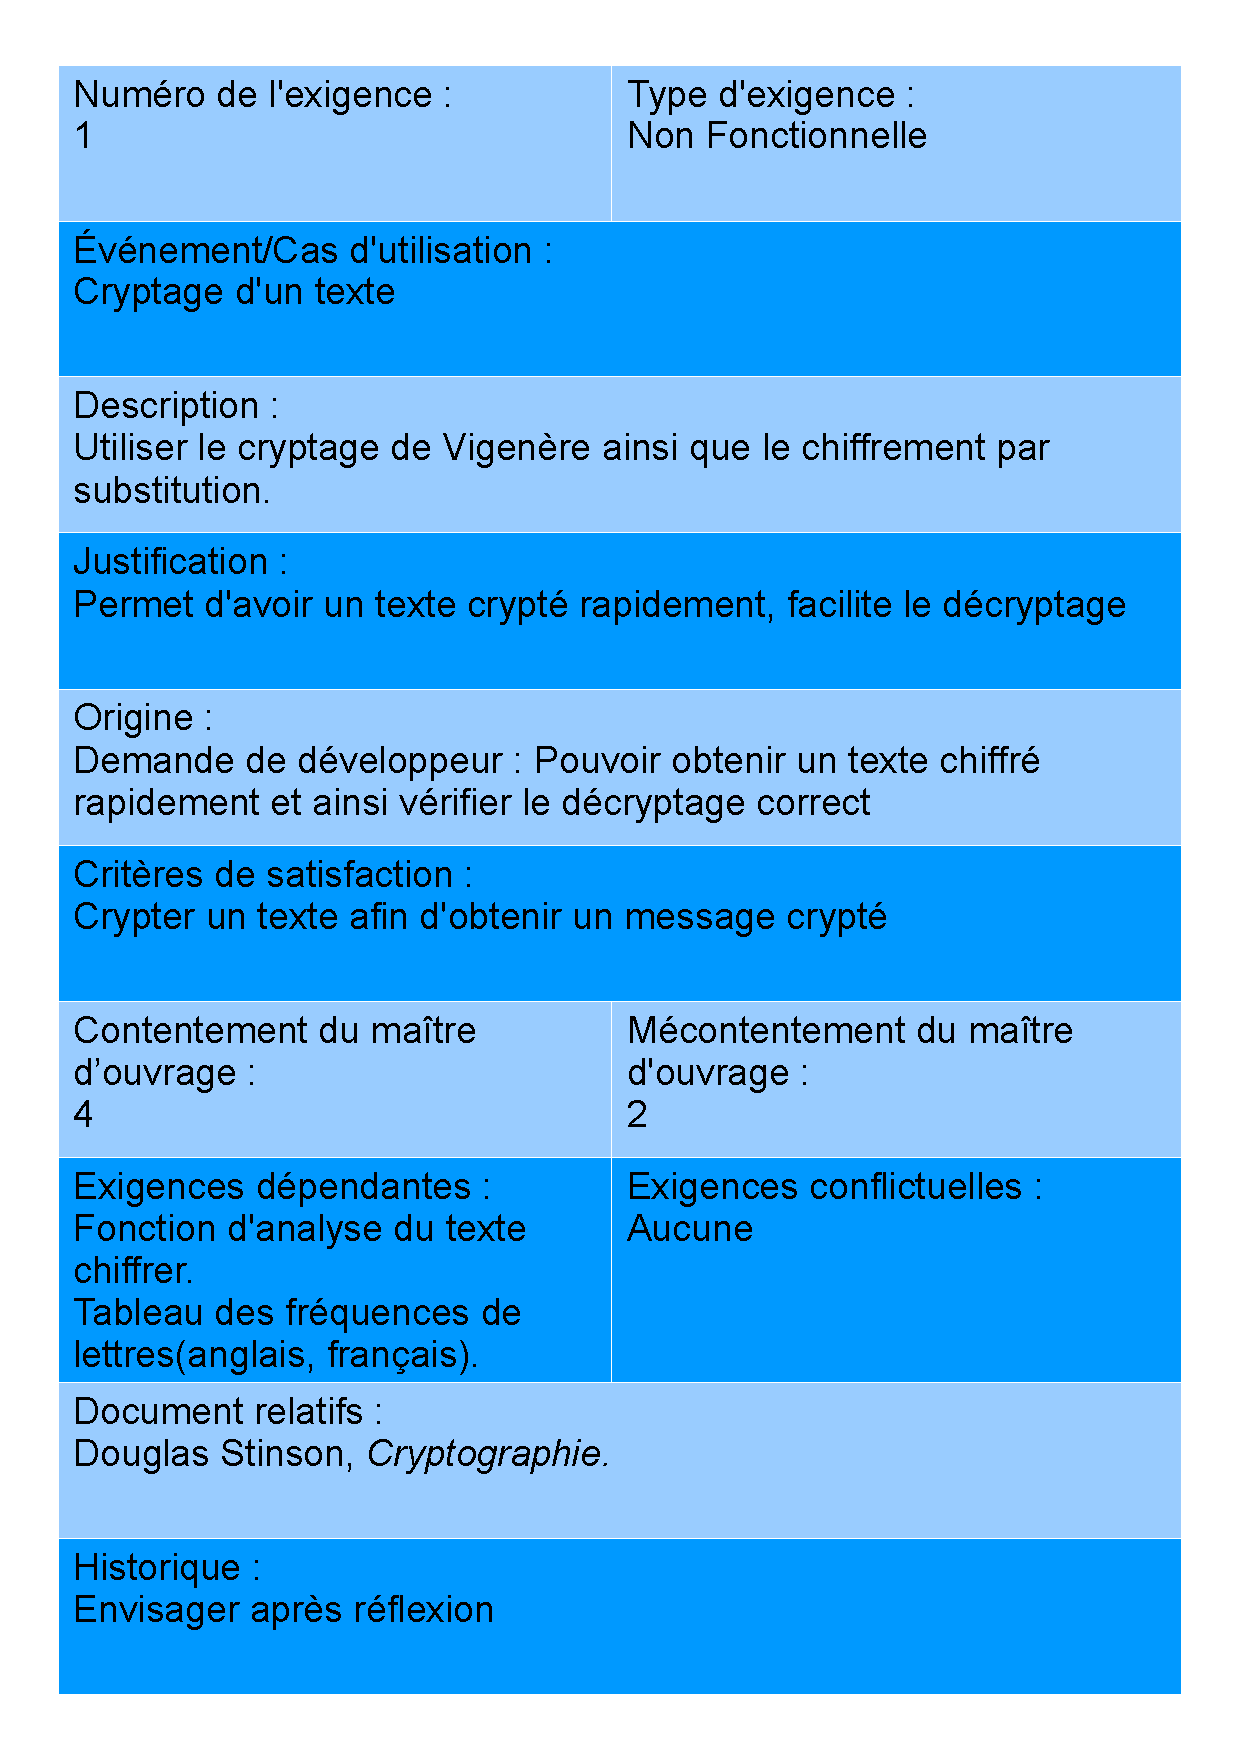
\includegraphics[scale=0.5,page = 1]{FichesExigences.pdf} \\
				\includegraphics[scale=0.5,page = 2]{FichesExigences.pdf} \\
				\includegraphics[scale=0.5,page = 3]{FichesExigences.pdf} \\
				\includegraphics[scale=0.5,page = 4]{FichesExigences.pdf} \\
				\includegraphics[scale=0.5,page = 5]{FichesExigences.pdf} \\
				\includegraphics[scale=0.5,page = 6]{FichesExigences.pdf} \\
				\includegraphics[scale=0.5,page = 7]{FichesExigences.pdf} \\
				\includegraphics[scale=0.5,page = 8]{FichesExigences.pdf} \\
				\includegraphics[scale=0.5,page = 9]{FichesExigences.pdf} \\
				\includegraphics[scale=0.5,page = 10]{FichesExigences.pdf} \\
				\includegraphics[scale=0.5,page = 11]{FichesExigences.pdf} \\
				\includegraphics[scale=0.5,page = 12]{FichesExigences.pdf} \\
				\includegraphics[scale=0.5,page = 13]{FichesExigences.pdf} \\
				\includegraphics[scale=0.5,page = 14]{FichesExigences.pdf} \\
				\includegraphics[scale=0.5,page = 15]{FichesExigences.pdf} \\
				\includegraphics[scale=0.5,page = 16]{FichesExigences.pdf} \\
				\includegraphics[scale=0.5,page = 17]{FichesExigences.pdf} \\
		\section{numerotation des exigences}
				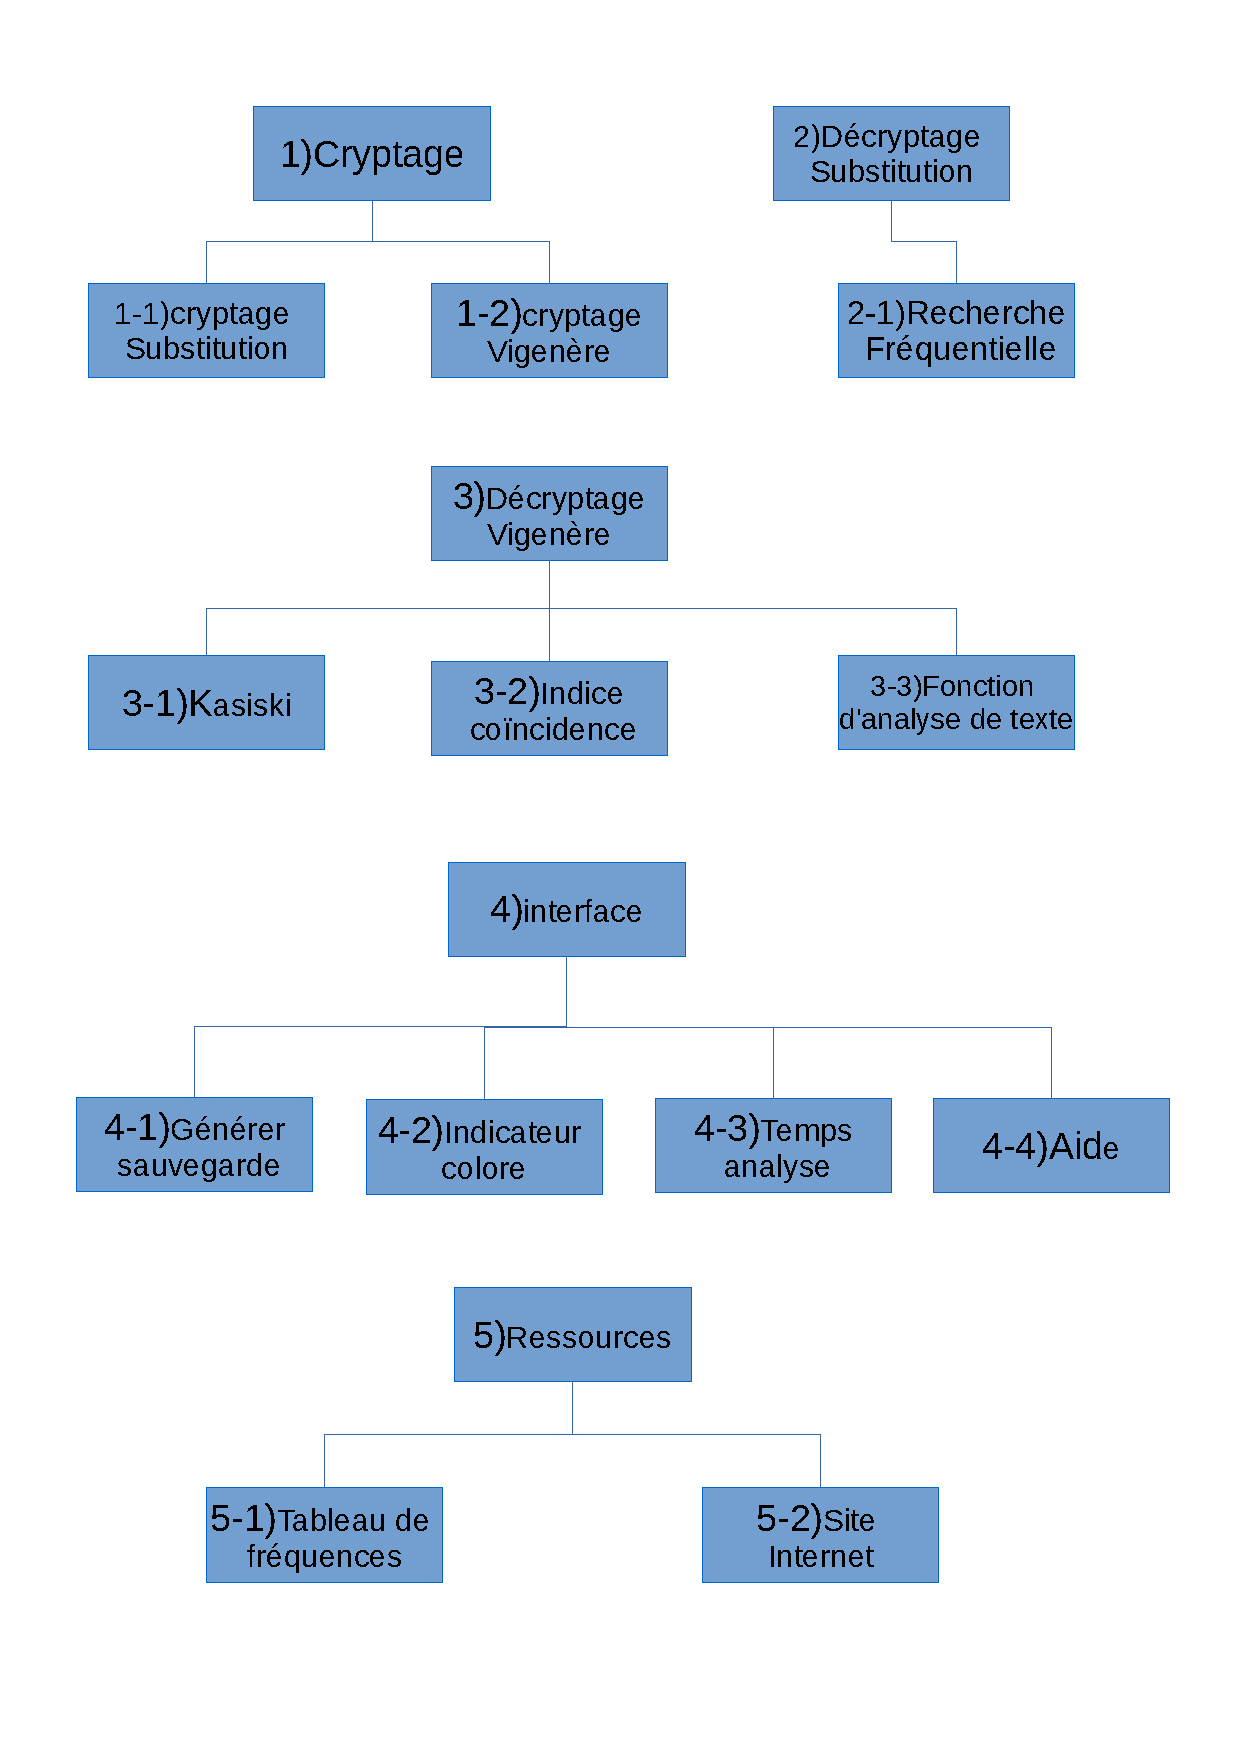
\includegraphics[scale=0.5]{Untit.pdf} \\
		
	\section{fondament du projet}
		\subsection{But Du Projet} 
			\subsubsection{Probleme de l'utilisation ou contexte du projet}
				Dans le cadre de notre L3 nous devons concevoir un programme d'aide au decryptage.
				Grace a notre programme le client/professeur va evaluer notre travail.
			\subsubsection{objectif de la section}
				L'objectif de ce module est de nous apprendre a travailler en equipe pour fournir un travail commun.
			\subsubsection{objectif du projet}
				Le but du projet est de realiser un automayique d'aide au décryptage, capable de retrouver une grande partie du texte d'origin a partir d'un texte chiffré. Il devra etre capable de déchiffré le chiffrement de vignère et le chiffrement par substitution.
		\subsection{personnes et organismes impliqués dans les enjeux du projet} 
			\subsubsection{maitre d'ouvrage}
				Ce projet fait partie du module projet de la 3eme annee d'info dirigé par Mme Kloul qui travaille pour l'uvsq.			
		\subsection{utilisateurs du produit}
			
	\section{contraintes sur le projet}
		\subsection{contraintes imposées non negociables} 
			\subsubsection{contraintes sur la conception de la solution}
				-Le produit doit permettre à l'utilisateur de décrypter une partie d'un message crypté.

				-Le produit doit crypter, décrypter un chiffrement de Vignère et un chiffrement par substitution.

				-Toutes les deadlines concernant l'application et son cahier des charges doivent être respectées.
			\subsubsection{Environnement de fonctionnement du système actuel }
				Le produit sera développé sous forme d'application. 
				Le programme s'appuiera essentiellement sur des recherches fréquentielles pour décrypter un chiffrement par substitution et utiliser le test de Kasiski et les indices de coincidences pour déchiffrer vigenère le message.
			\subsubsection{Lieux de fonctionnement prévus}
				Le produit étant une application, il faudra un ordinateur afin de le lancer.
				Il est préférable que l'utilisateur utilise un ordinateur moderne pour sa rapidité et sa fluidité
			\subsubsection{ De combien de temps les développeurs disposent-ils pour le projet ?}
				La deadline pour les développeurs est le Vendredi 12 Juin 2017.
			\subsubsection{ Quel est le budget affecté au projet ?}
				Le client ne nous a pas référé son budget.
		\subsection{Glossaire et conventions de dénomination}
			Cette section donne les définitions de tous les termes et acronymes utilisés dans le projet.

			k est la clé

			m est la taille de la clé

			n est la taille de message chiffré
			
			Les personnages Alice et Bob sont des figures classiques en cryptologie. Ces noms sont utilisés au lieu de « personne A » et « personne B » ; Alice et Bob cherchent dans la plupart des cas à communiquer de manière sécurisée.
			Alice est la personne qui envoie le message.
			Bob est celui qui veut recevoir le message.
			Oscar est celui qui essaye d'attaquer le message.
		\subsection{Faits et hypothèses utiles}	
			\subsubsection{Facteurs influençant le produit, mais qui ne sont pas des contraintes imposées sur les 				exigences}
	
				-Mettre en place une interface facile d'utilisation sur l'application de manière a ce que même 					un enfant puisse lancer le décryptage.
	\section{EXIGENCES FONCTIONNELLES}
		\subsection{Portée du travail}
			\subsubsection{la situation actuelle}
				Nous n'avons aucune base pour notre application, nous allons la crée de toutes pieces.
			\subsubsection{contenu du travail}
				Il est nécessaire de connaitre le chiffrement et le déchiffrement (avec et sans clé) de 				Vigenère et de substitution.
		\subsection{Portée du produit : cas d’utilisation}
			\subsubsection le diagramme de cas d'utilisation \\
				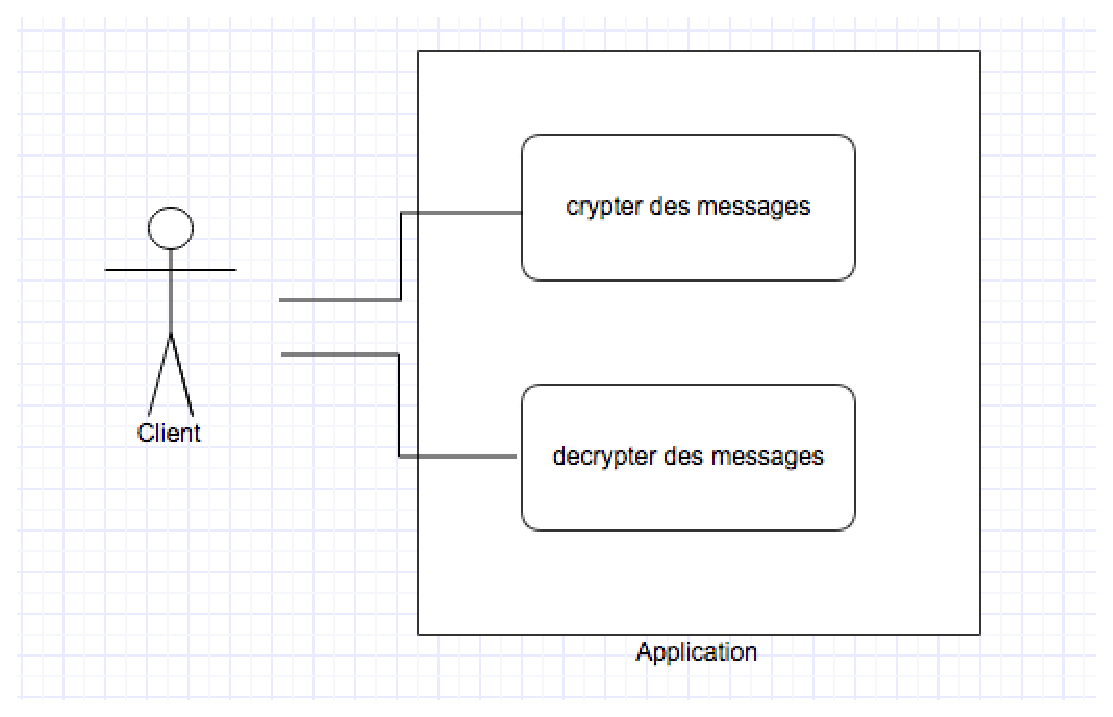
\includegraphics[scale=0.5]{dia.eps} \\
			\subsubsection description de ce diagramme
				Dans cette application il n'ya qu'un seul type d'utilisateur qui est le client 
				et qui peut crypter et decrypter avec deux methode differentes
		\subsection{Exigences fonctionnelles et exigences sur les données}
			\subsubsection Exigences fonctionnelles
				?????je crois quil faut mettre les numeros des exigences fonctionnelles (pas sur)
			subsub Exigences sur les données???? 
	\section{EXIGENCES NON FONCTIONNELLES}
		\subsection{Ergonomie et convivialité du produit}
			\subsubsection l'interface
				L'interface permettera de rentrer facilement le texte à décrypter, par copier coller par 				exemple.
				L'interface permettera de choisir la langue (anglais, français) grâce à un simple menu 					déroulant.
				L'interface permettera d'afficher facilement le resultat obtenu.
			\subsubsection Le style du produit
				le programme sera évaluer par la résponsable du module Projet de la L3 donc il doit apparaître 					simple et effiace (pas de superflu).
				Le programme ne doit pas etre trop gros en terme de resolution, on doit pouvoir l'afficher sur 					tous les types d'écran d'ordinateur.

		\subsection{Facilité d’utilisation et facteurs humains}
			\subsubsection Facilité d'utilisation
				Le programme sera simple à utiliser pour un adulte.

				Le programme pourra etre utilisé par des personnes sans qu'ils y soient formés.
			\subsubsection Personnalisation et internationalisation
				Le programme sera trop simple pour etre personnalisable et il sera en anglais.
			\subsubsection Facilité d'apprentissage
				-Le developpement d'un site web présentant le produit ainsi que toutes ces carectéristiques. 				Ce site web pourra également disposer d'un forum permettant aux internautes de proposer certaines 				amélioration à faire sur l'application et également critiquer certaines fonctionnalités de 					l'application.
				Il sera possible au grand public d’utiliser le programme sans formation.
			\subsubsection facilité d' compréhension et politesse
				Le produit devrait utiliser des symboles et des mots naturellement compréhensibles par les
				utilisateurs potentiels.
				Le produit doit cacher les détails de sa construction à l’utilisateur.

		\subsection{Fonctionnement du produit}
			\subsubsection Rapidité d’exécution et temps de latence
				La réponse sera assez rapide pour éviter d’interrompre le flux de pensée de l’utilisateur.

			\subsubsection Précision et exactitude
				C'est un programme d'aide au décryptage donc il ne donnera jamais un texte complet en sortie 					mais un texte à trou rempli au mieux avec le resultats du décryptage.
			\subsubsection Fiabilité et disponibilité
				Le programme devrait être disponible pour une utilisation de 24 heures par jour et 365 jours
				par an. 

		\subsection{Adéquation du produit avec son environnement}
			\subsubsection Environnement physique prévu
				Le programme sera utilisé sur un ordinateur.
			\subsubsection Environnement technologique prévu
				Le programme pourra fonctionner sur Windows, Linux et a priori Mac.
			\subsubsection Approche « produit » prêt à être commercialisé
					Le programme sera distribué sous forme d'archive correspondant au système 						d'exploitation du client.
		\subsection{Maintenance, support, portabilité, installation du produit}
			\subsubsection Maintenance du produit
				Le système doit pouvoir être maintenu par des développeurs qui ne sont pas les
				développeurs d’origine.
				Mettre en place une gestion des erreurs ou bugs (par exemple a l'aide de tests unitaire, 				d'indicateurs comme des variables..etc).
			\subsubsection Conditions spéciales concernant la maintenance du produit
				Site internet avec des informations sur l'application.
				Permettre également un dialogue avec d'autres utilisateurs de la même application.
				Demandes d'aide au developpeur charger de la maintenance de l'application.
			\subsubsection Exigences en matière de support
				L'utilisateur doit pouvoir communiquer avec d'autres utilisateurs et/ou les developpeurs en 					charge de la maintenance.
			\subsubsection Exigences de portabilité
				L'application peut fonctionner sur plusieurs environnements car "un makefile est fourni et 				permet a l'utilisateur de build en fonction de son environnement"(commelinux, windows ou autre).
			\subsubsection Installation du système
				L'application doit pouvoir être installée très facilement sur n'importe quel environnement.
				Le site internet doit permettre de repondre a certaines interrogations.
		\subsection{Sécurité}
			\subsubsection Intégrité
				Definition d'un niveau d'importance de "l'exactitude" necessaire au dechiffrage du message.
				(exemple : les coordonnées pour envoyer un missile nucleaire doivent etre ultra precise)
			\subsubsection Protection des données à caractère personnel
				Message d'information a l'ouverture de l'application qui permet d'informer l'utilisateur des 					precautions a prendre.
			\subsubsection Audit et traçabilité
				Definition d'un repertoire de sauvegarde avec les dates des messages.
			\subsubsection Protection contre les infections
				Il faudra conserver les fichiers de maniere securisée et prudente ou alors les supprimer une 					fois que ce celui-ci n'a plus d'utilité.
		\subsection{Exigences culturelles et politiques}
			\subsubsection Exigences culturelles
				L'application pourra gerer plusieurs langues (plusieurs tableaux de frequencages de lettres).
			\subsubsection Exigence politiques
				L'application et notamment les informations obtenues via l'application devront être hermétique 					vis a vis de n'importe quel états/organisation. a supprimer????
			\subsection{Lois et standards influençant le produit}
			\subsubsection Conformité avec la loi
				Les informations personnelles seront soumises a la loi sur la protection des données
				personnelles (la loi informatique et libertés).
			\subsubsection Conformité avec des standards
La notion de conventions de codage (coding style) désigne un ensemble de règles et de conseils 
adoptés par les membres d’un projet logiciel pour écrire et mettre en forme du code.
Les conventions de codage visent essentiellement à améliorer la lisibilité du code : elles doivent 
permettre au programmeur d’identifier « du premier coup d’œil » un maximum de choses dans 
le  code, de se repérer facilement, de savoir ou trouver les choses, etc.Une fois adoptés, elles
facilitent grandement l’écriture, la maintenance et aident à éviter certaines erreurs.
Dès lors qu’on travaille sur un projet logiciel d’une certaine ampleur, qui plus est à
plusieurs, l’expérience montre qu’il est très important de se mettre d’accord sur les
conventions de codage.	\section{AUTRES ASPECTS DU PROJET}
		\subsection{Questions sans réponse}
		Nous pensons avoir abordé une grande partie des aspects du projet et es attentes du client.
		\subsection{COTS : progiciels et composants commerciaux}
		Il existe sur le marché pas mal de produits pouvant etre des solutions potentielles/de remplacement. En effet, 			sur internet
		("en ligne"), il existe des sites proposant de decrypter votre texte. Nous avons par exemple tester le site 			www.dcode.fr, qui
		pour le dechiffrement avec Vigenere, fonctionne trés bien.
		Il y'a aussi une application (Decrypto) sur le Google Play Store (parmi plusieurs applis),qui est gratuite et 			qui permet aussi de dechiffrer Vigenere par exemple.
		Enfin, on peut telecharger des logiciels gratuits comme Axcrypt. Des logiciels payants/privés existe surement 			a l'usage des
		professionnels ou encore des services de police spécialisés.
		\subsection{Nouveaux problèmes, créés par le nouveau système}
		-Il peut y avoir un probleme de place ou memoire lors de l'installation du "systeme" malgré que l'application 			soit legere.
		
		-Un ralentissement de "l'environnement" peut aussi etre constaté a la suite de l'utilisation du nouveau 			systeme.
		\subsection{Tâches à faire pour livrer le système}
		Phase I: Identification du projet : La demande du client est clarifiée, les objectifs précisés et dans sa 			globalité le projet (ou service a livrer) est identifié. De plus, les contraintes a respecter sont 				evaluées et la strategie de realisation est mise en place
		Phase II: Definition du projet : Son contenu est defini de maniere tres precise et la planification des 			echeances et de la repartition du travail est etablie.
		Phase III: Realisation : On realise le projet en adequation avec les exigences du clients et selon le plan de 			travail defini au prealable
		Phase IV: Finalisation : Le produit est evalué puis remis au client.
		
		
		
		\subsection{Contrôle final de qualité sur site (Cutover)}
		Controle final sur un texte test. Un texte chiffré par vigenere et par substitution seront preparés, ainsi que 			leur version dechiffrées. Le resultat de ceux-ci via l'utilisation de l'application sera comparé au resultat 				preparé "sur feuille". 
		\subsection{Risques liés au projet}
		Aprés utilisation de l'application, certains risques existent. En effet, une personne etrangère peut avoir 			acces a l'ordinateur et ainsi recuperer les fichiers decryptés telechargés.
		\subsection{Estimation des coûts du projet}
		 	Pour une estimation precise des coûts du projet il faut estimer le coût en taille, 
			le coût en charge de travail, le coût des délais et le prix. Dans ce projet on vas surtout 
			se concentrer sur la taille de l'application et donc détérminer son coût grace au nombre de 
			lignes de code (que l'on ne pouras détérminer qu'aprés avoir réfléchis sur l'architecture du 				programme).		  		
		\subsection{Manuel utilisateur et formations à envisager}
			L'utilisateur aura acces à un menu lui permettant de choisir de crypter ou décrypter un texte,
			puis la méthode qu'il veut utiliser pour ce faire (vignaire ou substitution), il ne lui restera 
			plus qu'a importer son texte.
		\subsection{Salle d’attente : idées pour les futures versions}
			Bien que le programme ait été demandé que pour les langues francaise et anglaise, 
			il sera sans doute possible d'ajouter d'autre langues dans des versions futurs. 
			Il pourras étre également possible d'ajouter une option permettant à l'utilisateur

			d'entrer un type de texte (poéme, roman, ordre militaire,...) pouvant aider au décryptage. Ou meme 				encore conserver un historique des "dechiffrements" ou aussi permettre a l'application de savoir 			directement si l'on va crypter ou decrypter un texte.

		\subsection{Idées de solutions}
		 	Il s'agiras de rentrer un nouvaux tableau de données pour chaque nouvelles langues et pour 
			chaque nouveau style.
			Au vu de l'agencement des caracteres dans le texte, l'application pourra savoir automatiquement quelle 				operation le client chercher a effectuer (cryptage ou decryptage).
\end{document}
